%% intro.tex
%%
%% Copyright 2017 Evandro Coan
%% Copyright 2012-2016 by abnTeX2 group at http://www.abntex.net.br/
%%
%% This work may be distributed and/or modified under the
%% conditions of the LaTeX Project Public License, either version 1.3
%% of this license or (at your option) any later version.
%% The latest version of this license is in
%%   http://www.latex-project.org/lppl.txt
%% and version 1.3 or later is part of all distributions of LaTeX
%% version 2005/12/01 or later.
%%
%% This work has the LPPL maintenance status `maintained'.
%% The Current Maintainer of this work is the Evandro Coan.
%%
%% The last Maintainer of this work was the abnTeX2 team, led
%% by Lauro César Araujo. Further information are available on
%% https://www.abntex.net.br/
%%
%% This work consists of a bunch of files. But originally there ware 3 files
%% which are renamed as follows:
%% Renamed the `abntex2-modelo-include-comandos` to `chapters/chapter_1.tex`
%% Renamed the `abntex2-modelo-trabalho-academico.tex` to `chapters/intro.tex`
%% Renamed the `abntex2-modelo-references.bib` to `aftertext/modelo-ufsc-references.bib`
%%
%% This file was originally the main template file, however this main file was
%% split into several new files, which are respectively drastically changed,
%% except this files which contains most of the main documentation message.
%%

% ------------------------------------------------------------------------
% ------------------------------------------------------------------------
% abnTeX2: Modelo de Trabalho Academico (tese de doutorado, dissertacao de
% mestrado e trabalhos monograficos em geral) em conformidade com
% ABNT NBR 14724:2011: Informacao e documentacao - Trabalhos academicos -
% Apresentacao
% ------------------------------------------------------------------------
% ------------------------------------------------------------------------


% The \phantomsection command is needed to create a link to a place in the document that is not a
% figure, equation, table, section, subsection, chapter, etc.
%
% When do I need to invoke \phantomsection?
% https://tex.stackexchange.com/questions/44088/when-do-i-need-to-invoke-phantomsection
\phantomsection


% Is it possible to keep my translation together with original text?
% https://tex.stackexchange.com/questions/5076/is-it-possible-to-keep-my-translation-together-with-original-text
\chapter{\lang{Introduction}{Introdução}}
%\phantomsection
Trajectory similarity measuring has received significant attention in the last few years, and several measures have been proposed {to deal either with raw trajectories or semantic trajectories}. A \emph{raw trajectory} is generally represented as a sequence of points $T=<p_1, p_2, ...p_n>$, with $p_i=(x_i,y_i,t_i)$ where $x,y$ is the position of the object in space at time instant $t$.  Examples of similarity measures for raw trajectories are LCSS (Longest Common SubSequence) \cite{vlachos2002discovering}, EDR (Edit Distance on Real sequences) \cite{Chen:2005:RFS:1066157.1066213}, NWED (Normalized Weighted Edit Distance) \cite{dodge2012} and UMS (Uncertain Movement Similarity) \cite{Furtado-UMS-2018}. LCSS and EDR consider the sequence, but they force a match in all dimensions, not allowing partial similarity between trajectory points.
UMS is a parameter free method that considers only the spatial dimension, and it was developed to deal with data of varied or low sampling rate.


Existing works for raw trajectory similarity are limited to the spatio-temporal properties of raw trajectories, basically considering trajectories as data with only space information or space and time.

Similarity measures are the basis of several data processing and analysis techniques, such as information retrieval, location prediction, nearest neighbour queries, outlier detection, clustering, etc. A clustering algorithm, for instance, uses a similarity measure for grouping objects with similar trajectories. Outlier detection methods use similarity to find groups of trajectories with normal behavior, and the objects that are dissimilar to the majority, are the outliers. To detect specific trajectory patterns such as flocks \cite{Laube2005}, for instance, a raw trajectory similarity measure could be applied to find a minimal number of objects moving together in space and time.

In 2008 emerged the concept of semantic trajectories, introduced by \cite{Spaccapietra:2008:CVT:1347466.1347785}, where trajectories are represented as \emph{sequences of stops and moves}. \emph{Stops} are the most important parts of trajectories, representing the places that an object has visited for a minimal amount of time, and the \emph{moves} are the trajectory points between stops. In several works, stops are called points of interest (POIs), episodes, or stay points. Semantic trajectories are more complex than raw trajectories, because they have at least three dimensions: space, time, and semantics. {We consider in this thesis that semantics is any type of information associated to mobility data other than spatial location and time.}

The enrichment of trajectories with semantic information is a well studied topic in the literature, and a number of methods have been developed for this purpose, as the works of \cite{alvares2007model}, \cite{Palma2008}, \cite{manso}, and \cite{fileto2013baquara}. Applications as DayTag \cite{fernando2013} can detect stops and moves and the user can add the semantics to his/her trajectories. Examples of semantic information related to the stops can be, for instance, the name of the stop (e.g. Ibis Hotel) and the category (e.g. Hotel, Museum, Restaurant), while the semantic information related to the move could be, for instance, the name of the streets followed by the moving object and the category of the transportation mode. An example of semantic trajectory is shown in Figure \ref{fig:example_semantic_trajectory}.

With explosion of social media data, internet channels, and the facility to enrich trajectories with more context information as linked open data of Baquara \citep{fileto2013baquara}, allows the representation of movement in a more meaningful way. From social media data, for instance, a stop at a hotel can be enriched with the information of the number of stars, the price average, evaluation rate, facilities, parking, wifi, etc.  In this thesis we assume that semantic trajectories are represented as sequences of stops and moves, as originally defined in \cite{Spaccapietra:2008:CVT:1347466.1347785}, and the way how these trajectories are generated or enriched is out of the scope of this thesis.

\begin{figure}[h]
\centering
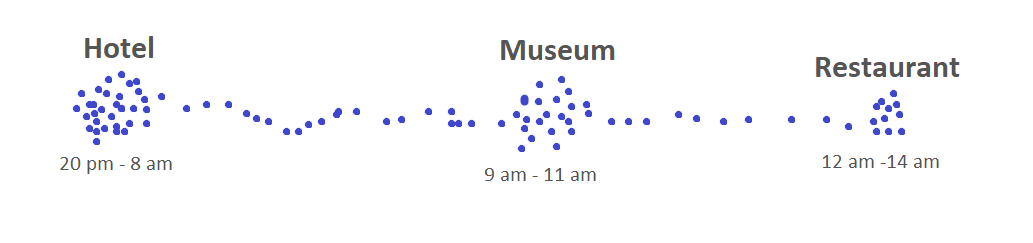
\includegraphics[width=1.0\textwidth]{Images/example_semantic-trajectory.png}
\caption{An example of a semantic trajectory}
\end{figure}
\label{fig:example_semantic_trajectory}

Similarity measures that consider both stops and moves can be important in a vast number of applications such as public transportation systems, traffic management, fraud detection, tourism, urban planning, car sharing, etc.


Only a few  similarity measures were proposed for semantic trajectories, as  \cite{Kang:2009:SMT:1529282.1529580}, \cite{Liu:2012:SMM:2442968.2442971}, \cite{Ying:2010:MUS:1867699.1867703}, and \cite{Furtado:TGIS12156}. The main problem of these measures is that they do not address all three dimensions (space, time, and semantics), as the works of \cite{Kang:2009:SMT:1529282.1529580} and \cite{Liu:2012:SMM:2442968.2442971}; or they exclusively address the stops, systematically ignoring all information about the moves, as the works of \cite{Ying:2010:MUS:1867699.1867703} and \cite{Furtado:TGIS12156}. To the best of our knowledge, none of the existing similarity measures for semantic trajectories have considered both stops and moves. The measure MSM (Multidimensional Similarity Measure) \cite{Furtado:TGIS12156}, for instance, considers only the stops, and they are treated as elements that are independent from each other, without considering the order/sequence as they appear in the trajectories. As MSM ignores the moves between stops, it can only be used to answer questions like: \emph{how similar are two trajectories $P$ and $Q$ considering their stops?}


\begin{figure}[h]
\centering
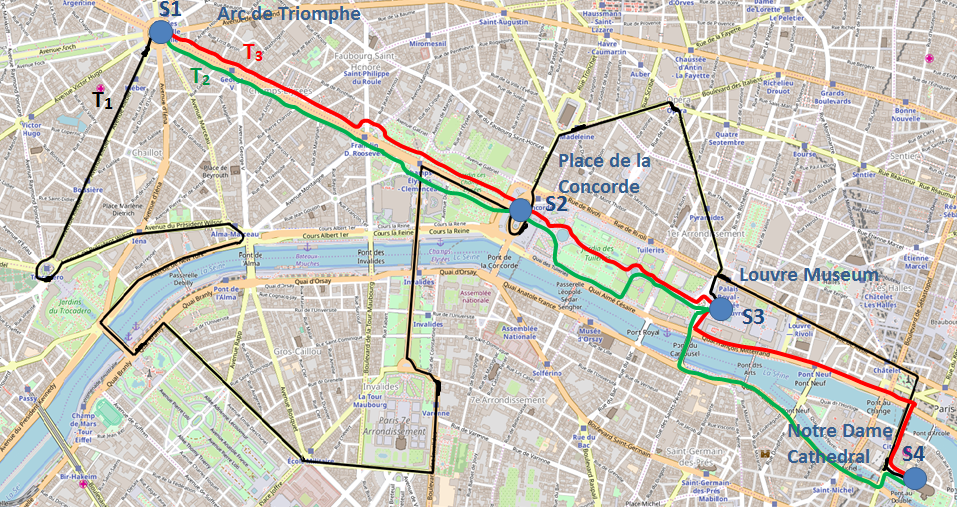
\includegraphics[width=1.0\textwidth]{Images/paris5.png}
\caption{Tourist trajectories in Paris with four stops}
\end{figure}
\label{fig:Paris}


{To better understand the need for considering both stops and moves in trajectory similarity analysis, let us consider the example in Figure \ref{fig:Paris}, for a tourism application, which shows three trajectories of tourists visiting Paris. These tourists visited four places, in this order:  Arc de Triomphe (first stop - S1), Place de la Concorde (second stop - S2), the Louvre Museum (third stop - S3), and the Notre Dame Cathedral (the last stop - S4). The three tourists visited the same places at the same order, but the tourists of trajectories $T2$ (green trajectory) and $T3$ (red trajectory) moved on foot, following the shortest path, while the tourist of trajectory $T1$ used a city tour hop on and hop off bus to appreciate the view. The question we want to answer in this thesis is \emph{how similar are trajectories $T1$, $T2$ and $T3$ considering both stops and moves?} From the figure it is clear that trajectories $T2$ and $T3$ are more similar, because they used almost the same paths between stops and moved on foot, while trajectory $T1$ has a spatially different move, performed with a different transportation mode. Now suppose that a tourism manager wants to recommend a trip to a new tourist arriving in Paris, and this new tourist wants to visit the same places visited by the tourists in the figure, but he wants to move on foot and follow the path used by the majority of the tourists.
For this case, we need to retrieve trajectories $T2$ and $T3$. 
Another example is the evaluation of the flow of tourists moving on foot between these four stops in order to eventually propose a new and direct hop on hop off tourist bus line.}

{In taxi fraud detection, for instance, a similarity measure will help to answer questions like: given two regions of interest, which is the standard path followed by the majority of the taxis and which are the outliers?
A real example of an outlier taxi trajectory is shown in Figure {\ref{fig:CRAWDAD_outlier}}, in the San Francisco dataset of the CRAWDAD project} \cite{epfl-mobility-20090224}. {In this example, given the stops Airport and  Westfield San Francisco Centre (WSFC), a similarity measure must consider both stops and moves to find the black trajectories as the most similar movements between the Airport and WSFC, and the trajectory in purple as the most dissimilar trajectory, which made a completely different and longer trip.}
 
\begin{figure}[h]
\centering
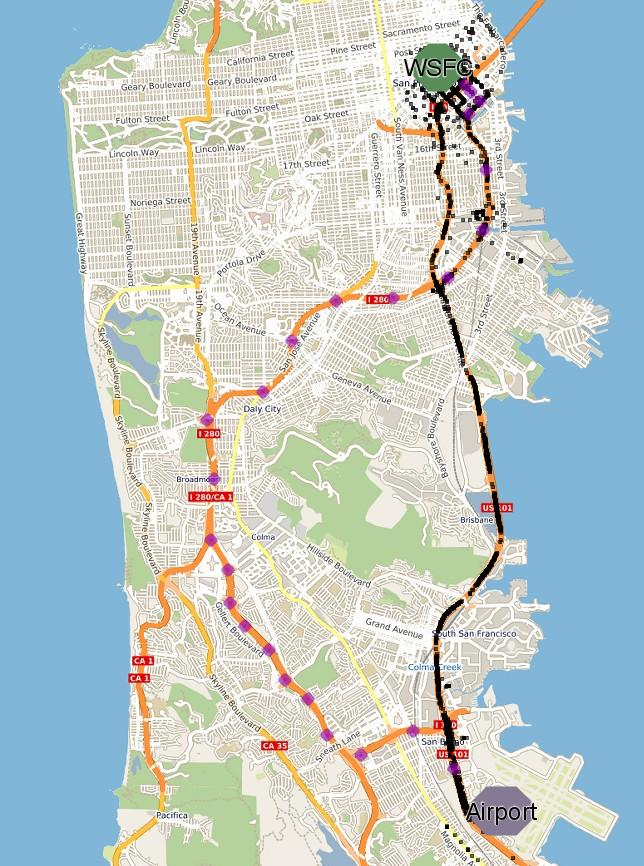
\includegraphics[width=0.5\textwidth]{Images/CRAWDAD-Outlier.jpg}
\caption{\label{fig:CRAWDAD_outlier} An outlier trajectory (in purple) going from Airport to downtown of San Francisco}
\end{figure}

In all previous examples, MSM cannot distinguish the trajectories, because it ignores the moves, and gives a similarity degree of 100\% for the trajectories in both scenarios.
Given the need of spatio-temporal similarity measures that consider both stops and moves, in this thesis we propose a new semantic trajectory similarity measure that extends MSM, proposed in \cite{Furtado:TGIS12156}, to support both stops and moves. Our approach considers the sequence of the stops, what is not supported by MSM, allows different semantics for the moves, and uses weights to provide importance degrees for stops, moves, and their attributes. 
In summary, we make the following contributions:
(i) we propose a new similarity measure for multidimensional sequences treating elements with heterogeneous dimensions, which is the case of stops and moves; (ii) the semantic similarity measure considers both \textit{stops} and \textit{moves}, as well as their space, time, and semantic dimensions, allowing the use of different distance functions for each dimension, making the measure robust for several applications; (iii) the measure is flexible enough to partially consider the order between stops and to support different weights for stops, moves, and dimensions, allowing to give more or less importance to different trajectory parts; (iv) we evaluate the proposed measure with experiments over synthetic and real data, comparing our proposal to a large number of measures developed either for raw or semantic trajectories.

\section{Objective}

The general objective of this thesis is the proposal of a novel semantic trajectory similarity measure, with proven accuracy and efficiency. We can further detail the aiming of this work in the following specific objectives:

\begin{itemize}
  \item The proposed similarity measure takes into account both \emph{stops} and \emph{moves} of the semantic trajectories;
  \item The proposed similarity measure allows the measuring of semantic trajectories considering their multiple dimensions, such as spatial, temporal, semantics, and other additional dimensions;
  \item The proposed similarity measure considers partially the sequence of the stops.
\end{itemize}

\section{Methodology}
The methodology adopted in this thesis has 8 steps:

\textit{Step} 1: Perform a review of the literature in related subjects such as trajectory similarity and semantic trajectory similarity using Google Scholar.

\textit{Step} 2: Study and implement related semantic trajectory similarity measures to find and understand limitations in related similarity measuring approaches.

\textit{Step} 3: Define a new semantic trajectory similarity measure to overcome limitations in existing similarity measures.

\textit{Step} 4: Select, organize, and pre-process datasets with real trajectory data, such as San Francisco taxi dataset from the CRAWDAD project\cite{epfl-mobility-20090224}, the Geolife dataset \cite{zheng2009mining}, and synthetic data, such as generated by Hermoupolis tool\cite{Pelekis-Hermoupolis}.

\textit{Step} 5: Evaluate the efficiency of the methods using the precision at recall \cite{BaezaYatesRibeiroNeto2011} as an information retrieval evaluation technique.

\textit{Step} 6: Comparison of the results obtained in all datasets with the most related approaches in literature.

\textit{Step} 7: Write an article describing the proposed semantic similarity measure, reporting the results of it evaluation.

\textit{Step} 8: Write the thesis describing the problem, the state-of-the-art, and the contribution for the problem solution with the advances over the state-of-the-art.

\section{Scope and Outline}

This thesis is limited to the proposal of a novel similarity measure for semantic trajectories, evaluation and comparison of this new similarity measure with the most related approaches in literature. 

The rest of this thesis is organized as follows: \textit{Chapter} \ref{sec:related} presents the basic concepts and the related works for this thesis, \textit{Chapter} \ref{sec:proposed_measure} presents the proposed similarity measure with a running example, \textit{Chapter} \ref{sec:experiments} presents experiments over real and synthetic trajectory data, \textit{Chapter} \ref{sec:discussion} presents a discussion about the choice of a measure in face of application problems, and \textit{Chapter} \ref{sec:conclusions} summarizes the contributions of this thesis, its limitations and points out future steps of the present research.
